

\begin{figure} [!htbp]
    \centering
    \begin{subfigure}[b]{1\textwidth}
        \centering
        \includegraphics[page=2, width=\textwidth]{98_Pictures/2025_02_ADAC Road to HANA_Org-Chart & Rollen_Realize-Phase.pdf}
        \caption{Organigramm R2H W1 2025}
         \label{fig:OrganigrammR2H2025}
    \end{subfigure}
    \hfill
    \begin{subfigure}[b]{1\textwidth}
        \centering
        \includegraphics[page=10,width=\textwidth]{98_Pictures/2026-04-13_W2_KickOff im neuen ProjektSetup.pdf}
        \caption{Organigramm R2H W2 2026}
         \label{fig:OrganigrammR2H2026}
    \end{subfigure}
    \caption{Organigramm R2H Projekt}
     \label{fig:OrganigrammR2H}
\end{figure}



\begin{figure} [!htbp]
    \centering
    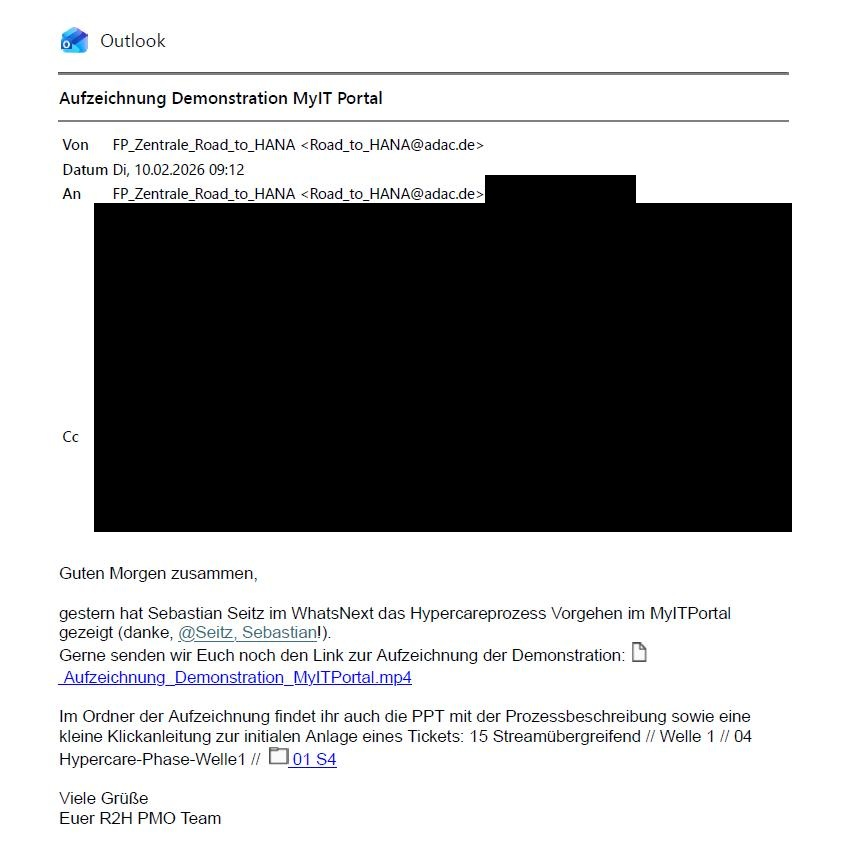
\includegraphics[width=0.99\textwidth]{98_Pictures/MyIt-Schulung.jpg}
    \caption{Programmschulung R2H im MyIT-Portal}
     \label{fig:ProgrammschulungMyIt}
\end{figure}

\begin{figure} [!htbp]
    \centering
    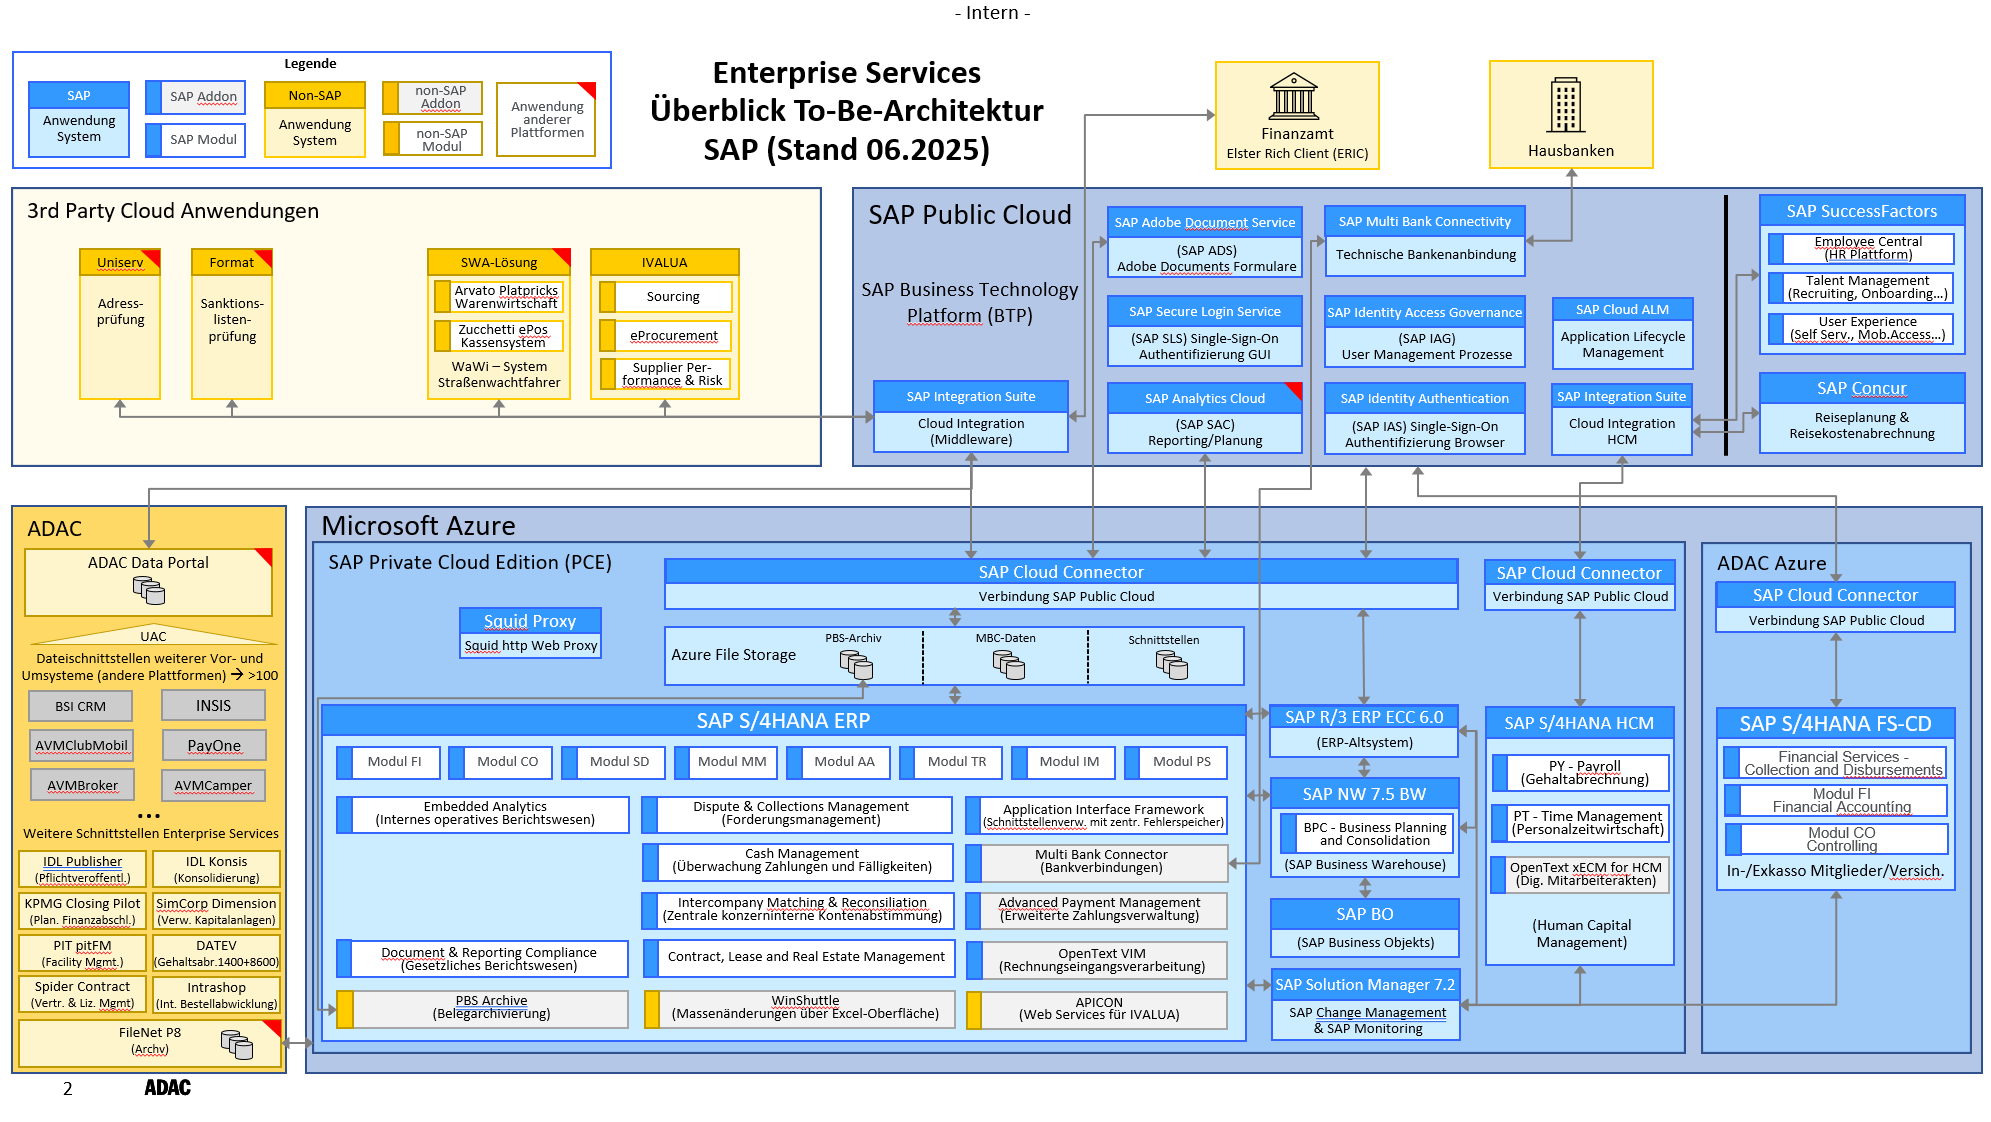
\includegraphics[width=0.99\textwidth]{98_Pictures/R2H_Interfaces_Integration.png}
    \caption{Interfaces und Integrationen von R2H}
     \label{fig:R2HInterfacesIntegration}
\end{figure}

\begin{figure} [!htbp]
    \centering
    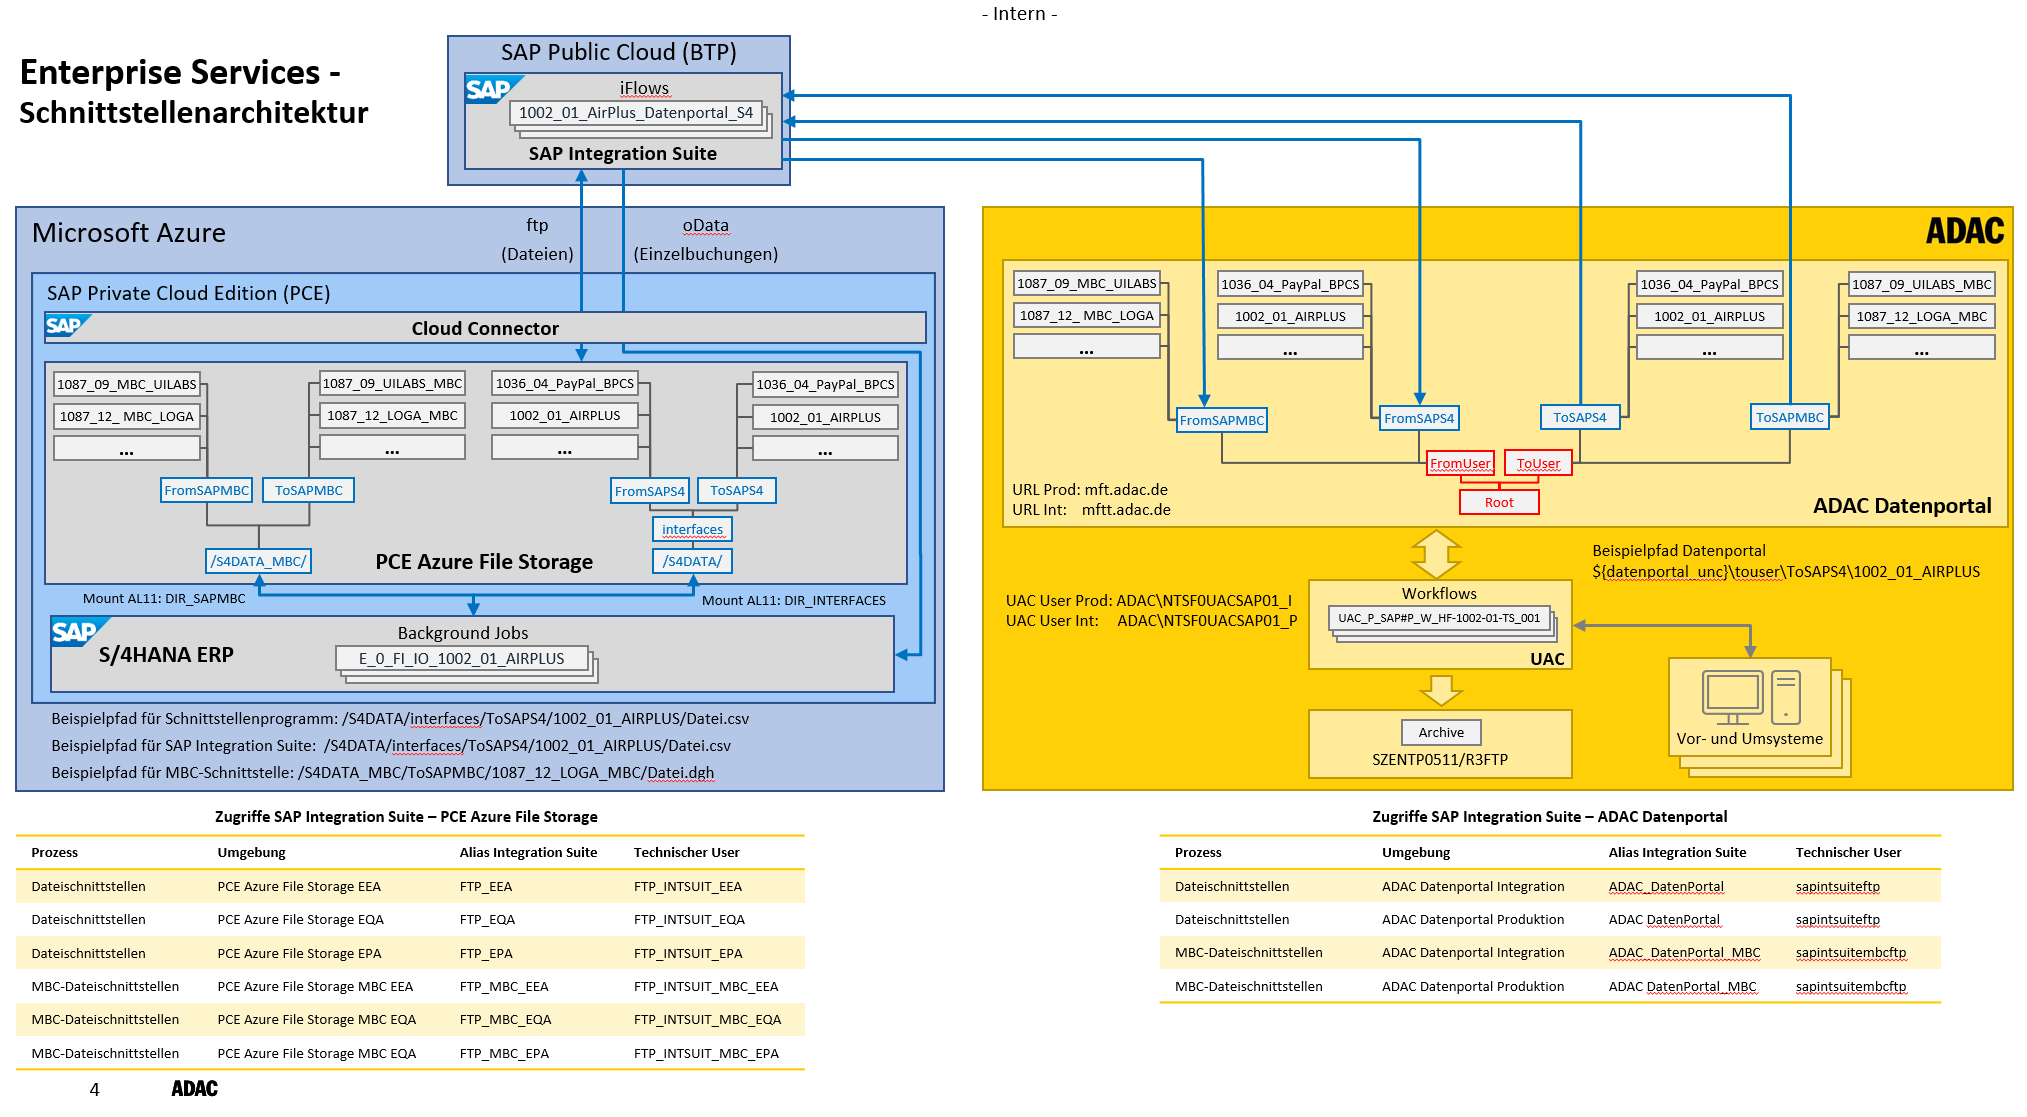
\includegraphics[width=0.99\textwidth]{98_Pictures/R2H_BFA_Detail.png}
    \caption{Detailansicht des implementierten BFA-Modells}
     \label{fig:R2HBFA}
\end{figure}

\clearpage
\newgeometry{top=1cm, bottom=1cm, left=1cm, right=1cm, head=0pt}
\begin{landscape}
\thispagestyle{empty}
\noindent\textit{Report - IPMA Level B}\hfill\textit{Sebastian Seitz}\hfill\textit{IPMA Level B}
\\[-0.9em]
\noindent\rule{\linewidth}{0.1pt}

\begin{figure} [!htbp]
    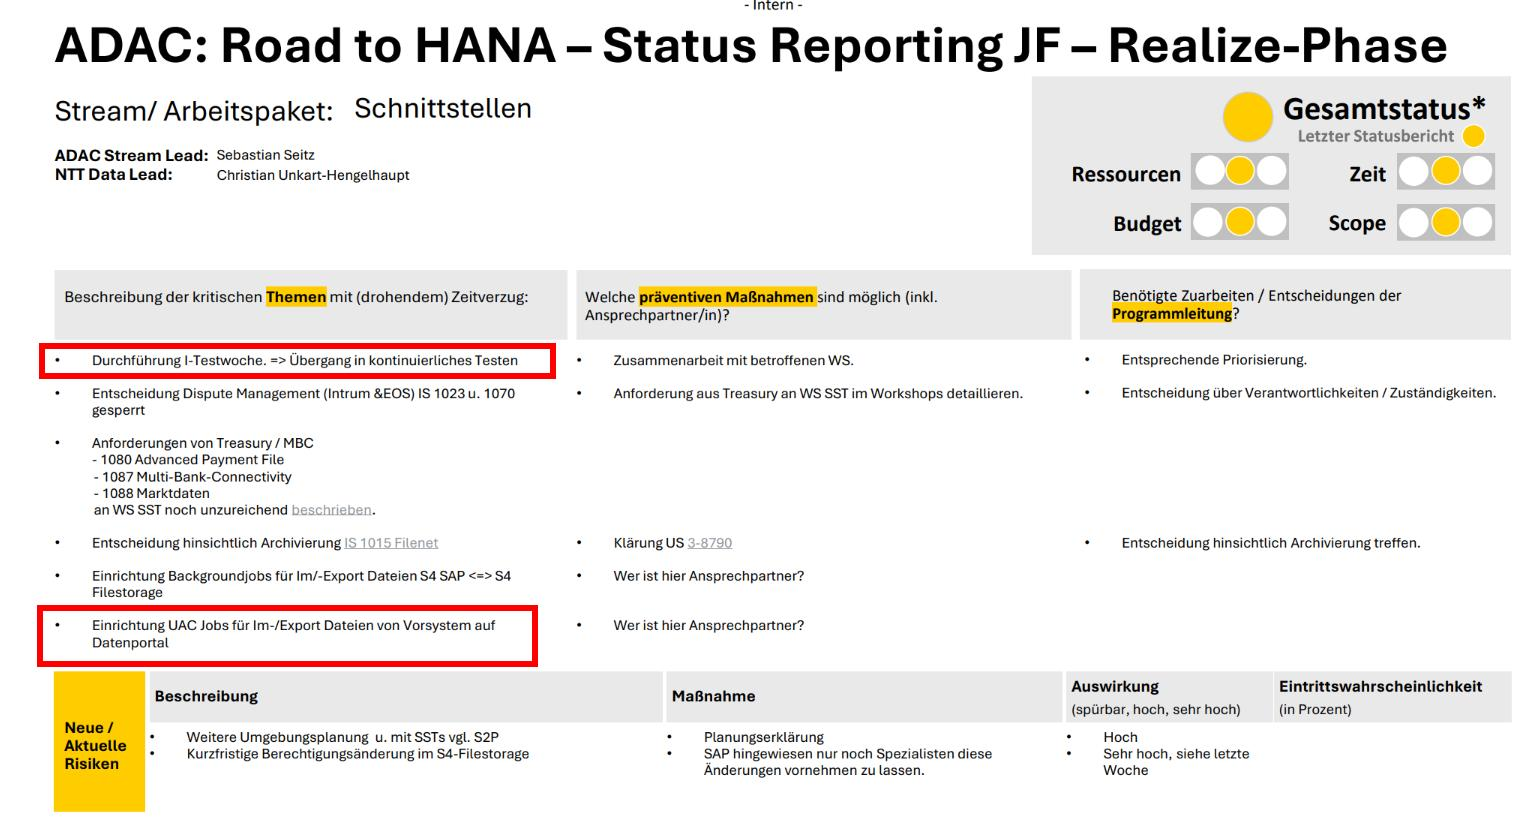
\includegraphics[width=0.99\textwidth]{98_Pictures/260610_StatusFolienSST.jpg}
    \caption{Statusfolie Juni 2025 SST Stand}
     \label{fig:R2HStatusSSTJuni2025}
\end{figure}

\vfill
\par\noindent\rule{\linewidth}{0.1pt}\\[-0.6em]
\noindent\textit{\curse}\hfill\textit{Seite \pagemark{}}
\end{landscape}
\restoregeometry
\clearpage

\begin{figure} [!htbp]
    \centering
    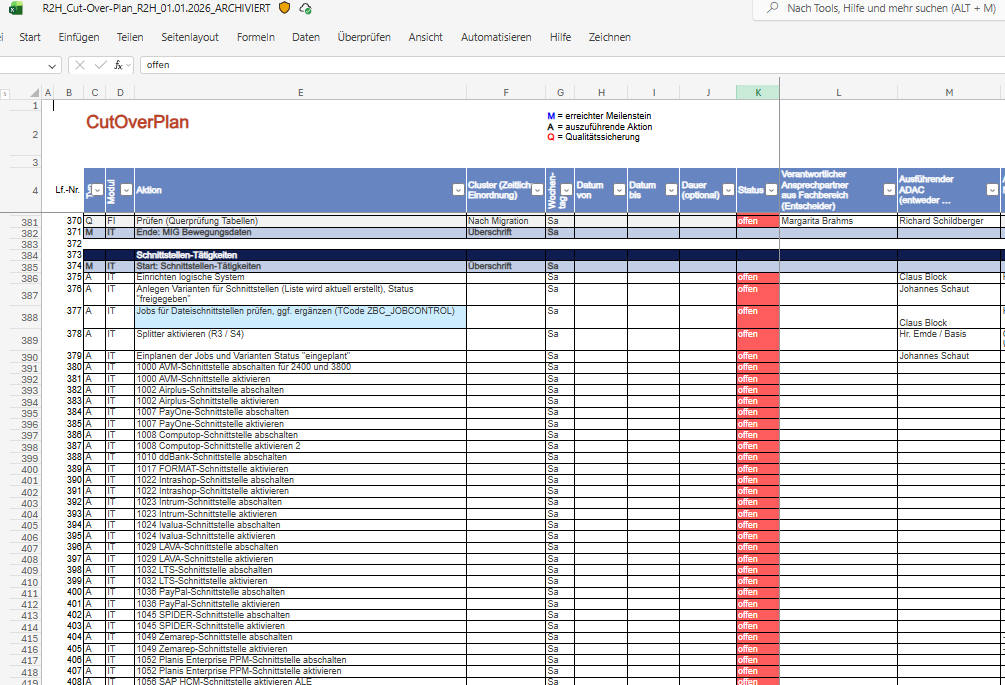
\includegraphics[width=0.99\textwidth]{98_Pictures/CutOverNtt.png}
    \caption{\acrshort{cop} \acrshort{gu} \acrshort{ricefw}}
     \label{fig:CutOverPlanGU}
\end{figure}

\begin{figure} [!htbp]
    \centering
    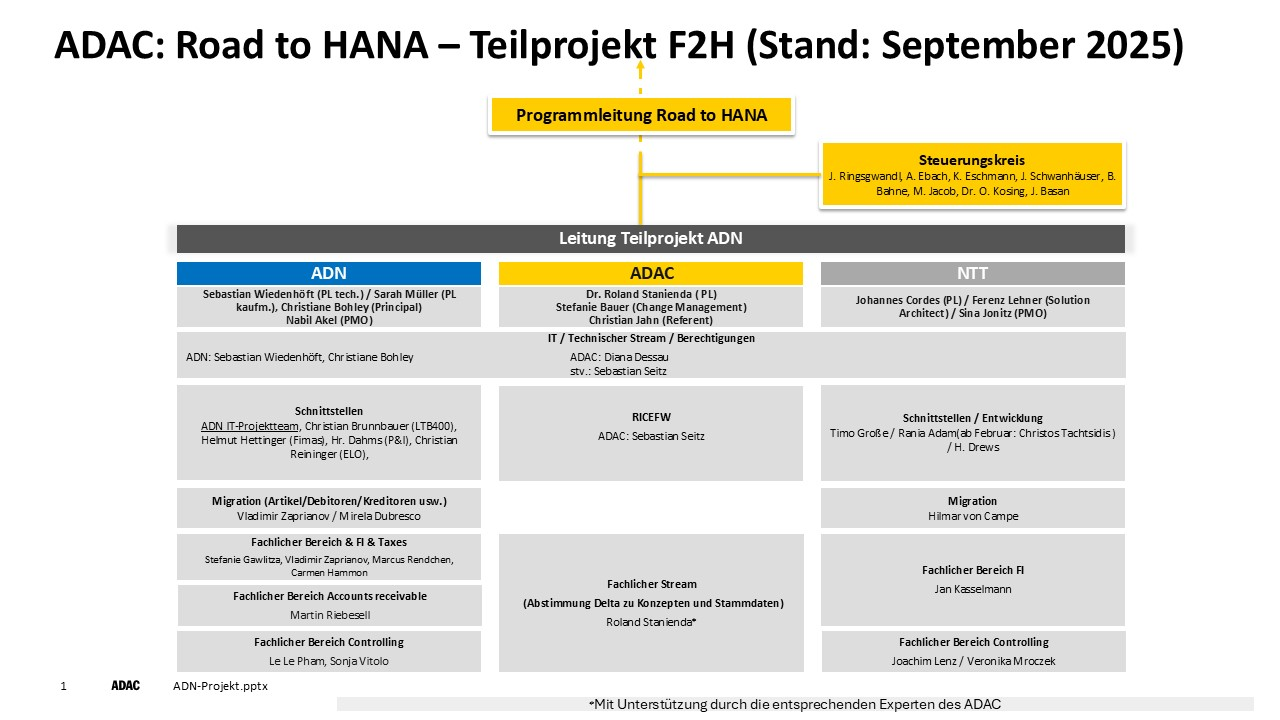
\includegraphics[width=0.99\textwidth]{98_Pictures/F2H_Organigramm_ADN_NTT_ADAC.jpg}
    \caption{Organigramm F2H Projekt}
     \label{fig:F2HOrganigramm}
\end{figure}

\begin{figure} [!htbp]
    \centering
    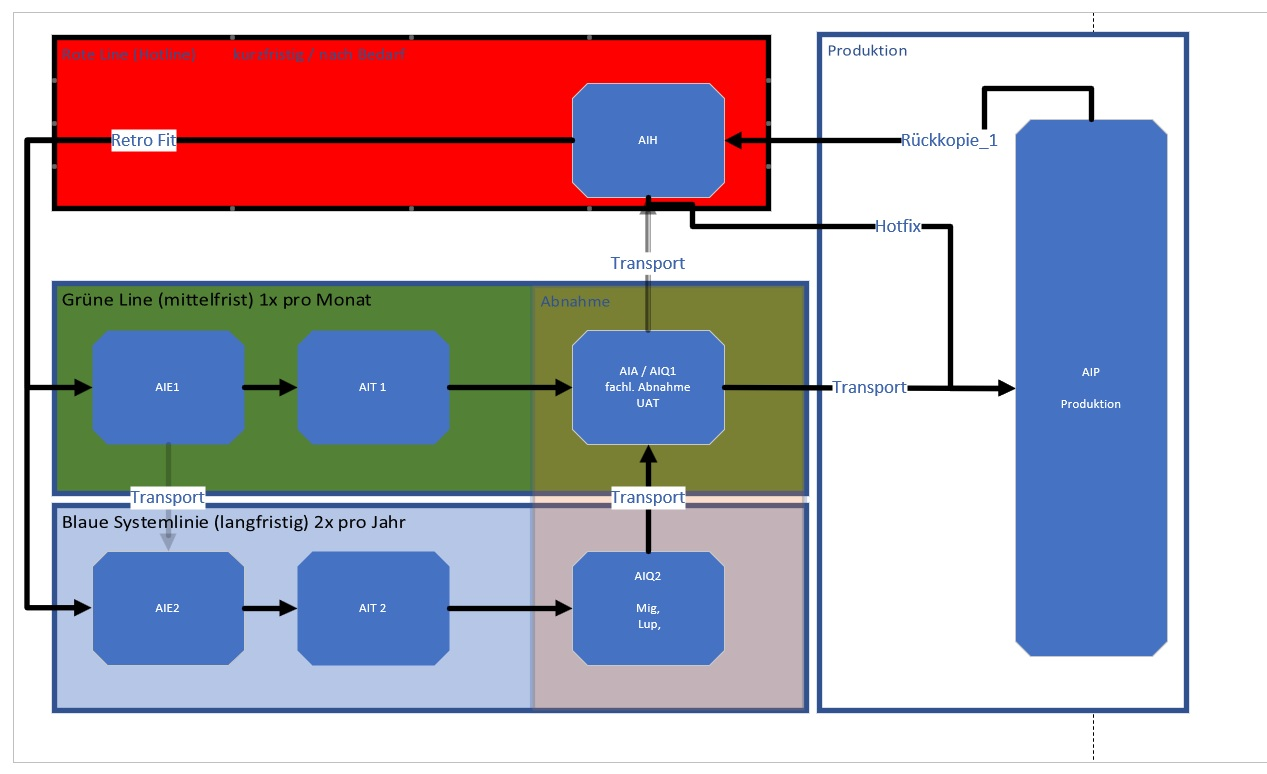
\includegraphics[width=0.99\textwidth]{98_Pictures/SAPUmgebungszielbild.jpg}
    \caption{Zielbild der \acrshort{erp}-SAP-Umgebungslandschaft}
     \label{fig:SAPUmgebungszielbild}
\end{figure}

\noindent
\begin{minipage}[t]{0.49\textwidth}
    \centering
    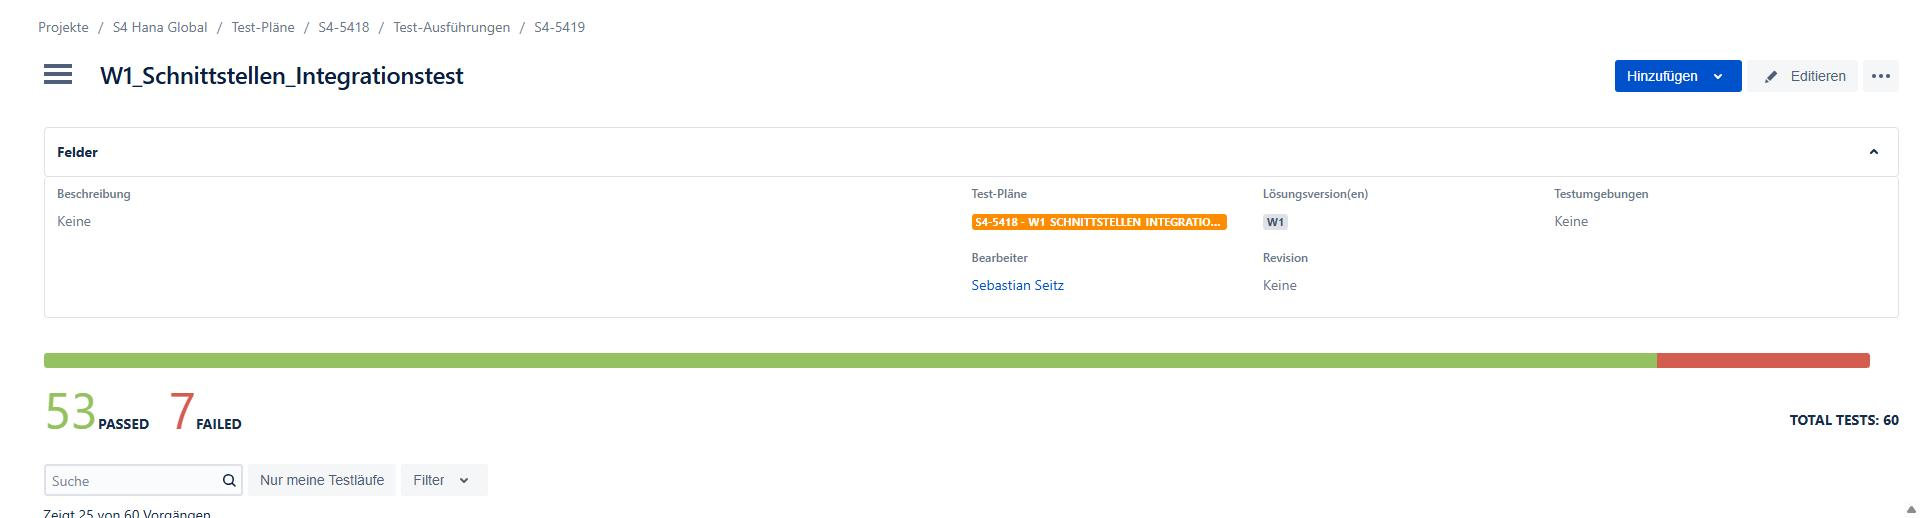
\includegraphics[width=\textwidth]{98_Pictures/TestpläneSST.jpg}
    \captionof{figure}{Testpläne \acrshort{sst}}
    \label{fig:TestpläneSST}
\end{minipage}
\hfill
\begin{minipage}[t]{0.49\textwidth}
    \centering
    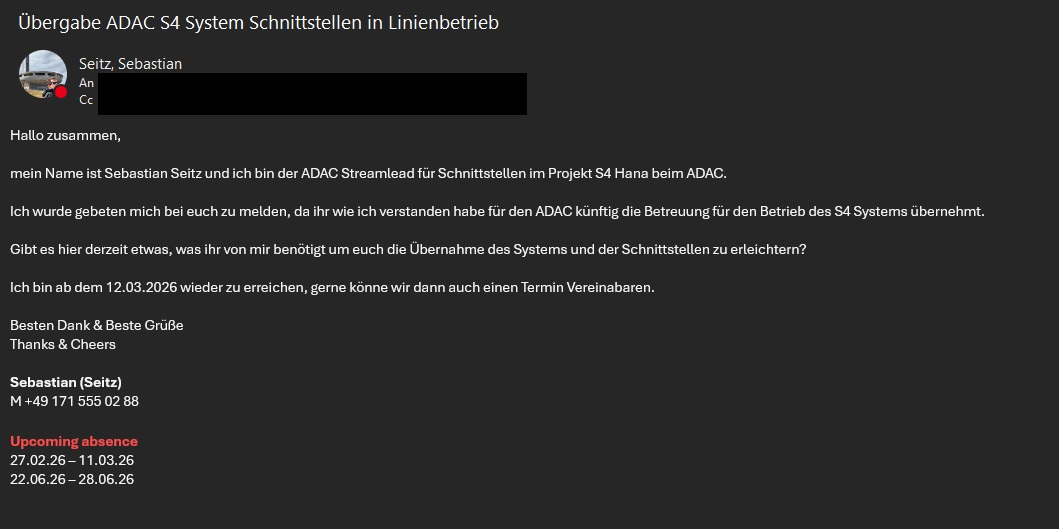
\includegraphics[width=\textwidth]{98_Pictures/InitiierungÜbergabe.jpg}
    \captionof{figure}{Initiierung Betriebsübergabe}
    \label{fig:InitiierungBetriebsübergabe}
\end{minipage}

\begin{figure} [!htbp]
    \centering
    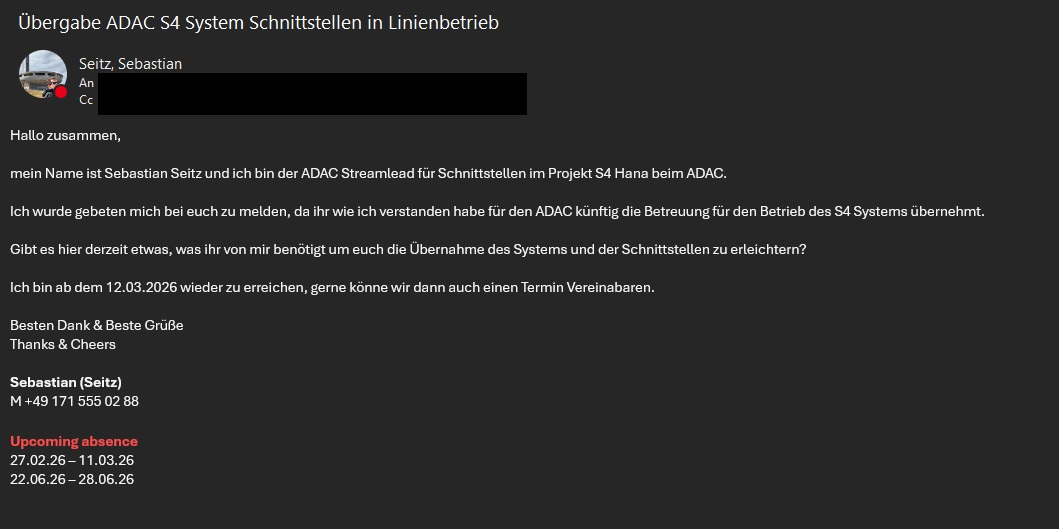
\includegraphics[width=0.99\textwidth]{98_Pictures/InitiierungÜbergabe.jpg}
    \caption{Initiierung und Übergabe}
     \label{fig:InitiierungÜbergabe}
\end{figure}

\begin{figure} [!htbp]
    \centering
    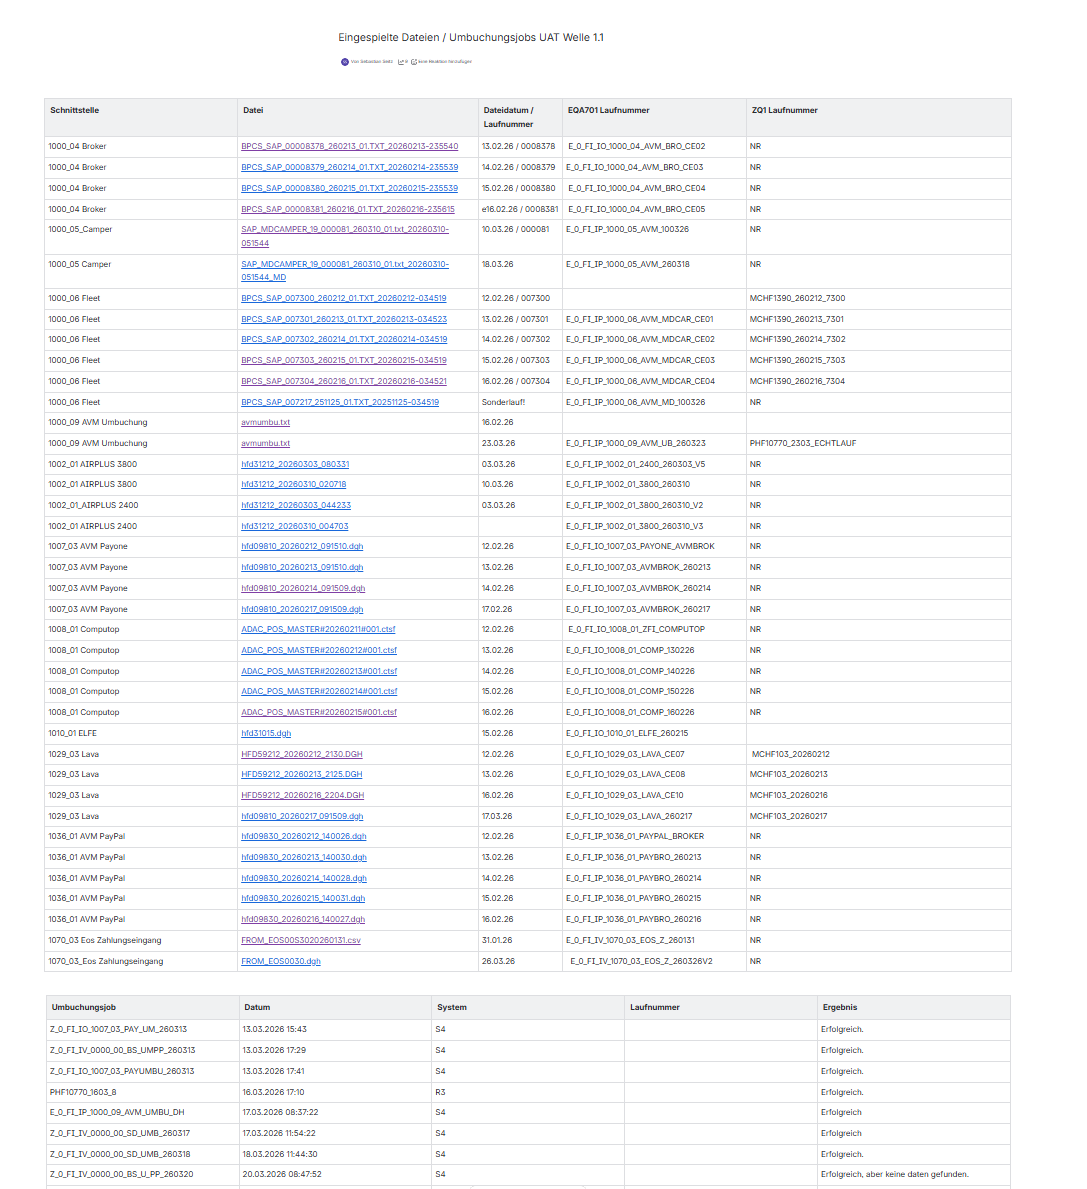
\includegraphics[width=0.99\textwidth]{98_Pictures/UAT_DatenDoku.png}
    \caption{UAT W1.1 Datendokumentation}
     \label{fig:UATDatenDoku}
\end{figure}

\begin{figure} [!htbp]
    \centering
    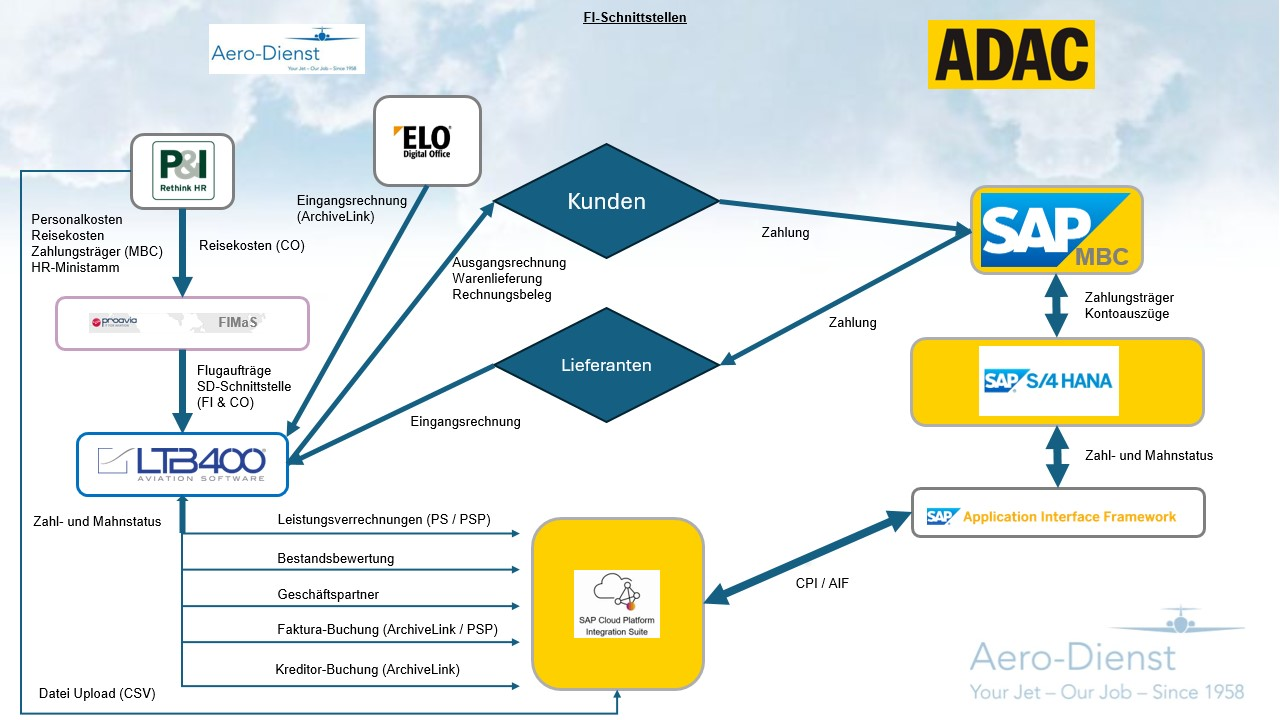
\includegraphics[width=0.99\textwidth]{98_Pictures/ADN_SST_FI.jpg}
    \caption{ADN SST FI Architekturbild}
     \label{fig:ADNSSTFI}
\end{figure}

\begin{figure} [!htbp]
    \centering
    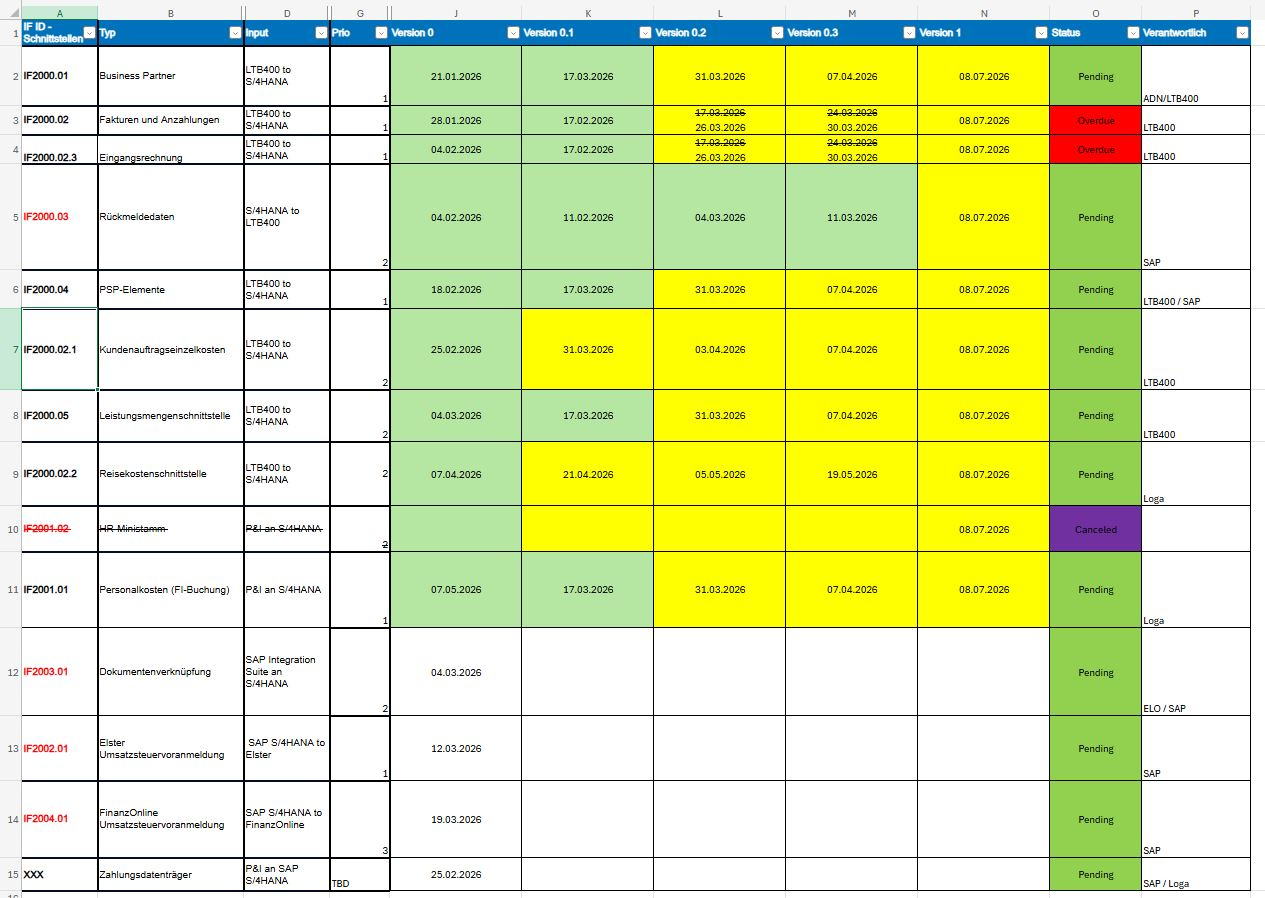
\includegraphics[width=0.99\textwidth]{98_Pictures/VersionsIterationSSTADN.JPG}
    \caption{ADN SST FI Versions- und Iterationsplan}
     \label{fig:VersionsIterationSSTADN}
\end{figure}

\begin{figure} [!htbp]
    \centering
    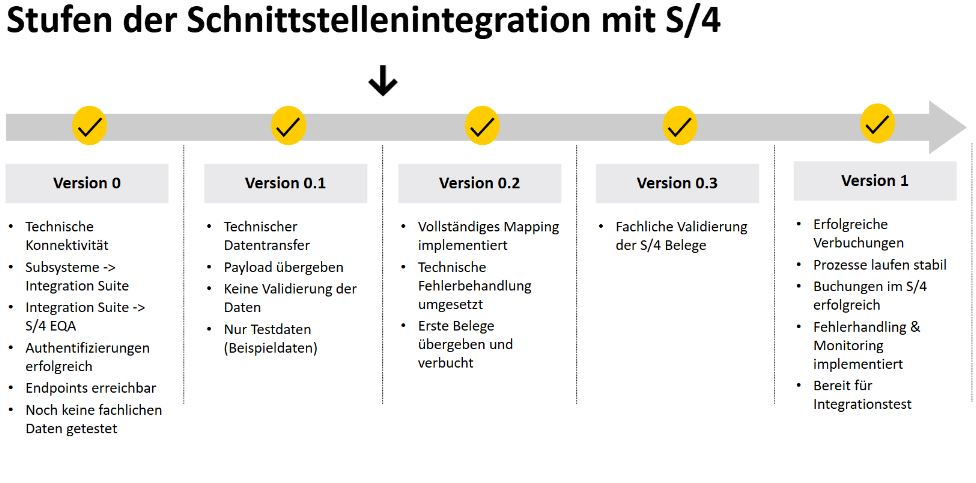
\includegraphics[width=0.99\textwidth]{98_Pictures/StufenIterationErklärung.JPG}
    \caption{ADN SST FI Versions- und Iterationsplan Erklärung}
     \label{fig:StufenIterationErklärung}
\end{figure}

\begin{figure} [!htbp]
    \centering
    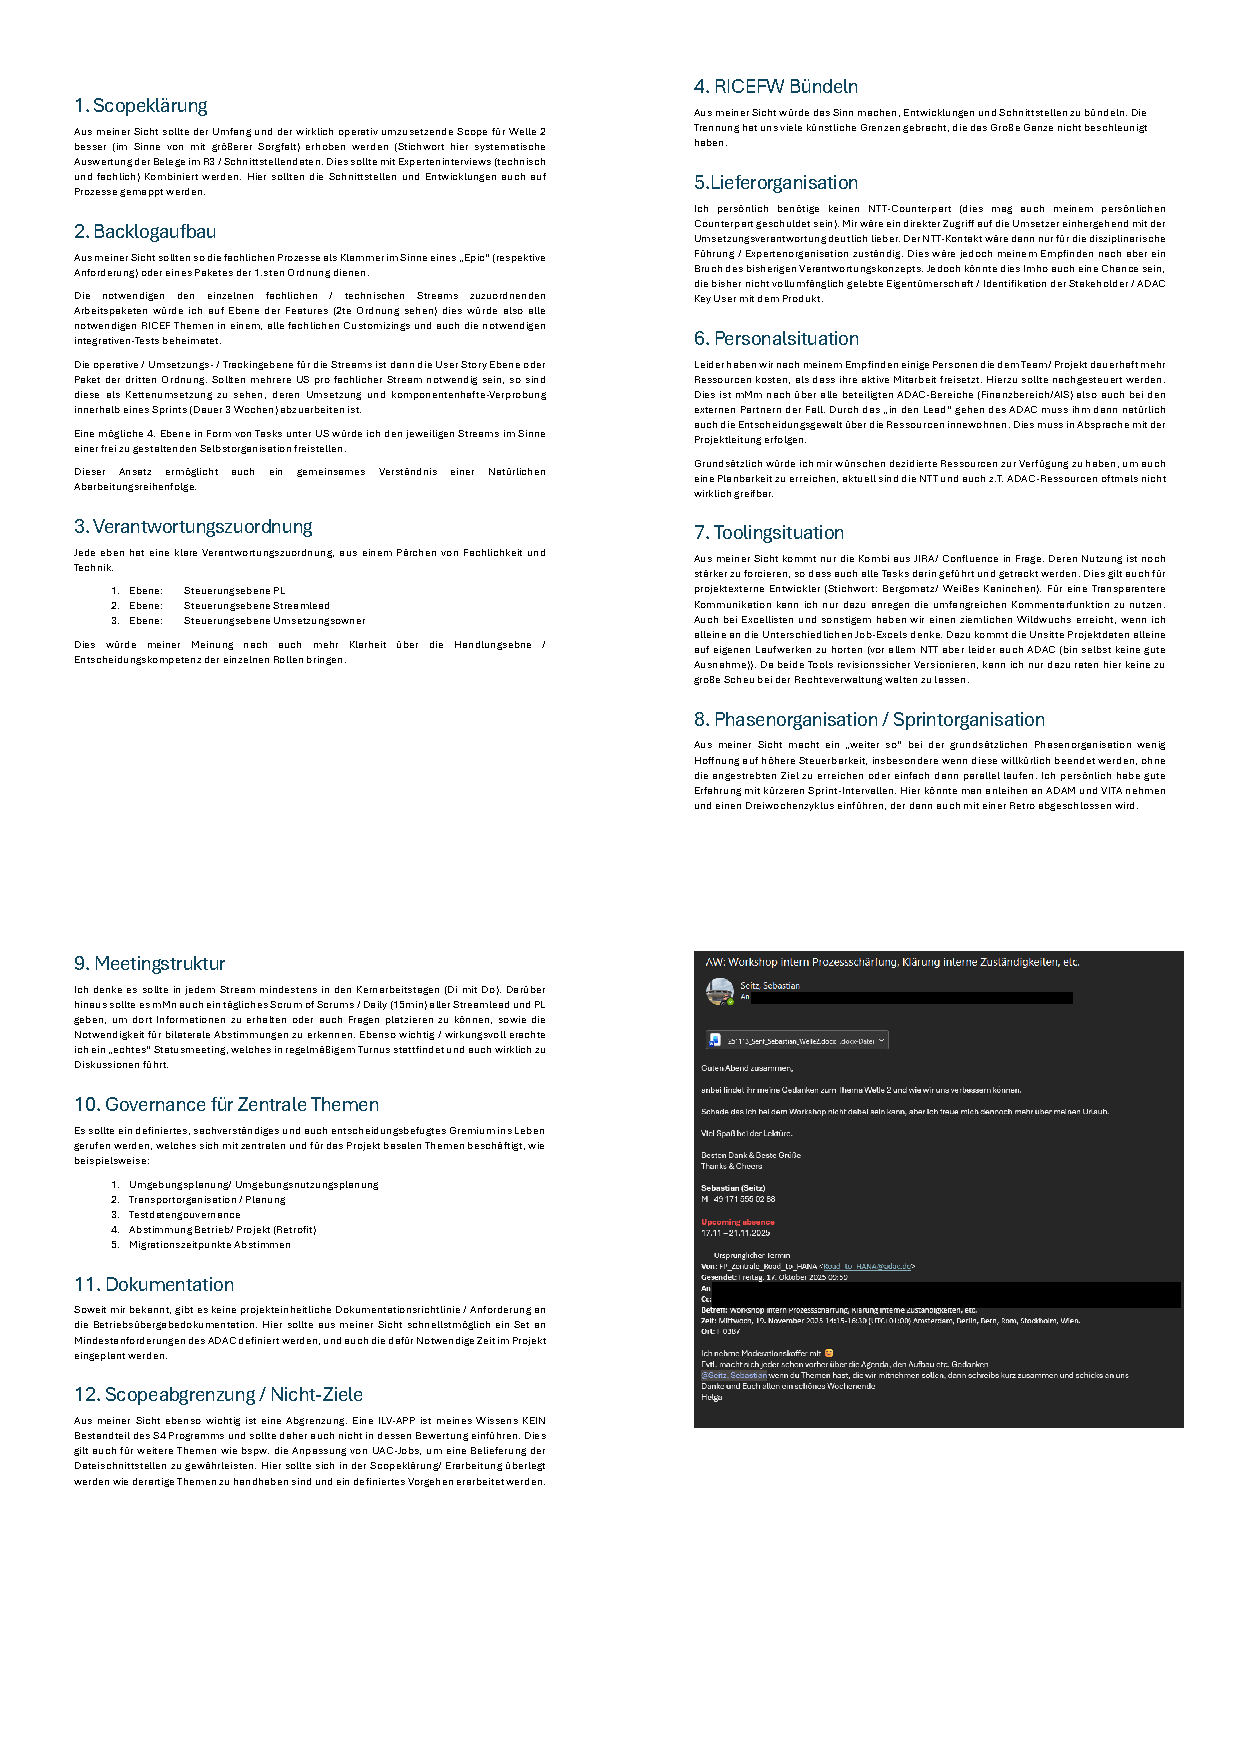
\includegraphics[width=0.99\textwidth]{98_Pictures/251113_Senf_Sebastian_Welle2.pdf}
    \caption{Anregungen W2 und Lessons Learned W1}
     \label{fig:AnregungenW2undLessonsLearnedW1}
\end{figure}

\begin{figure} [!htbp]
    \centering
    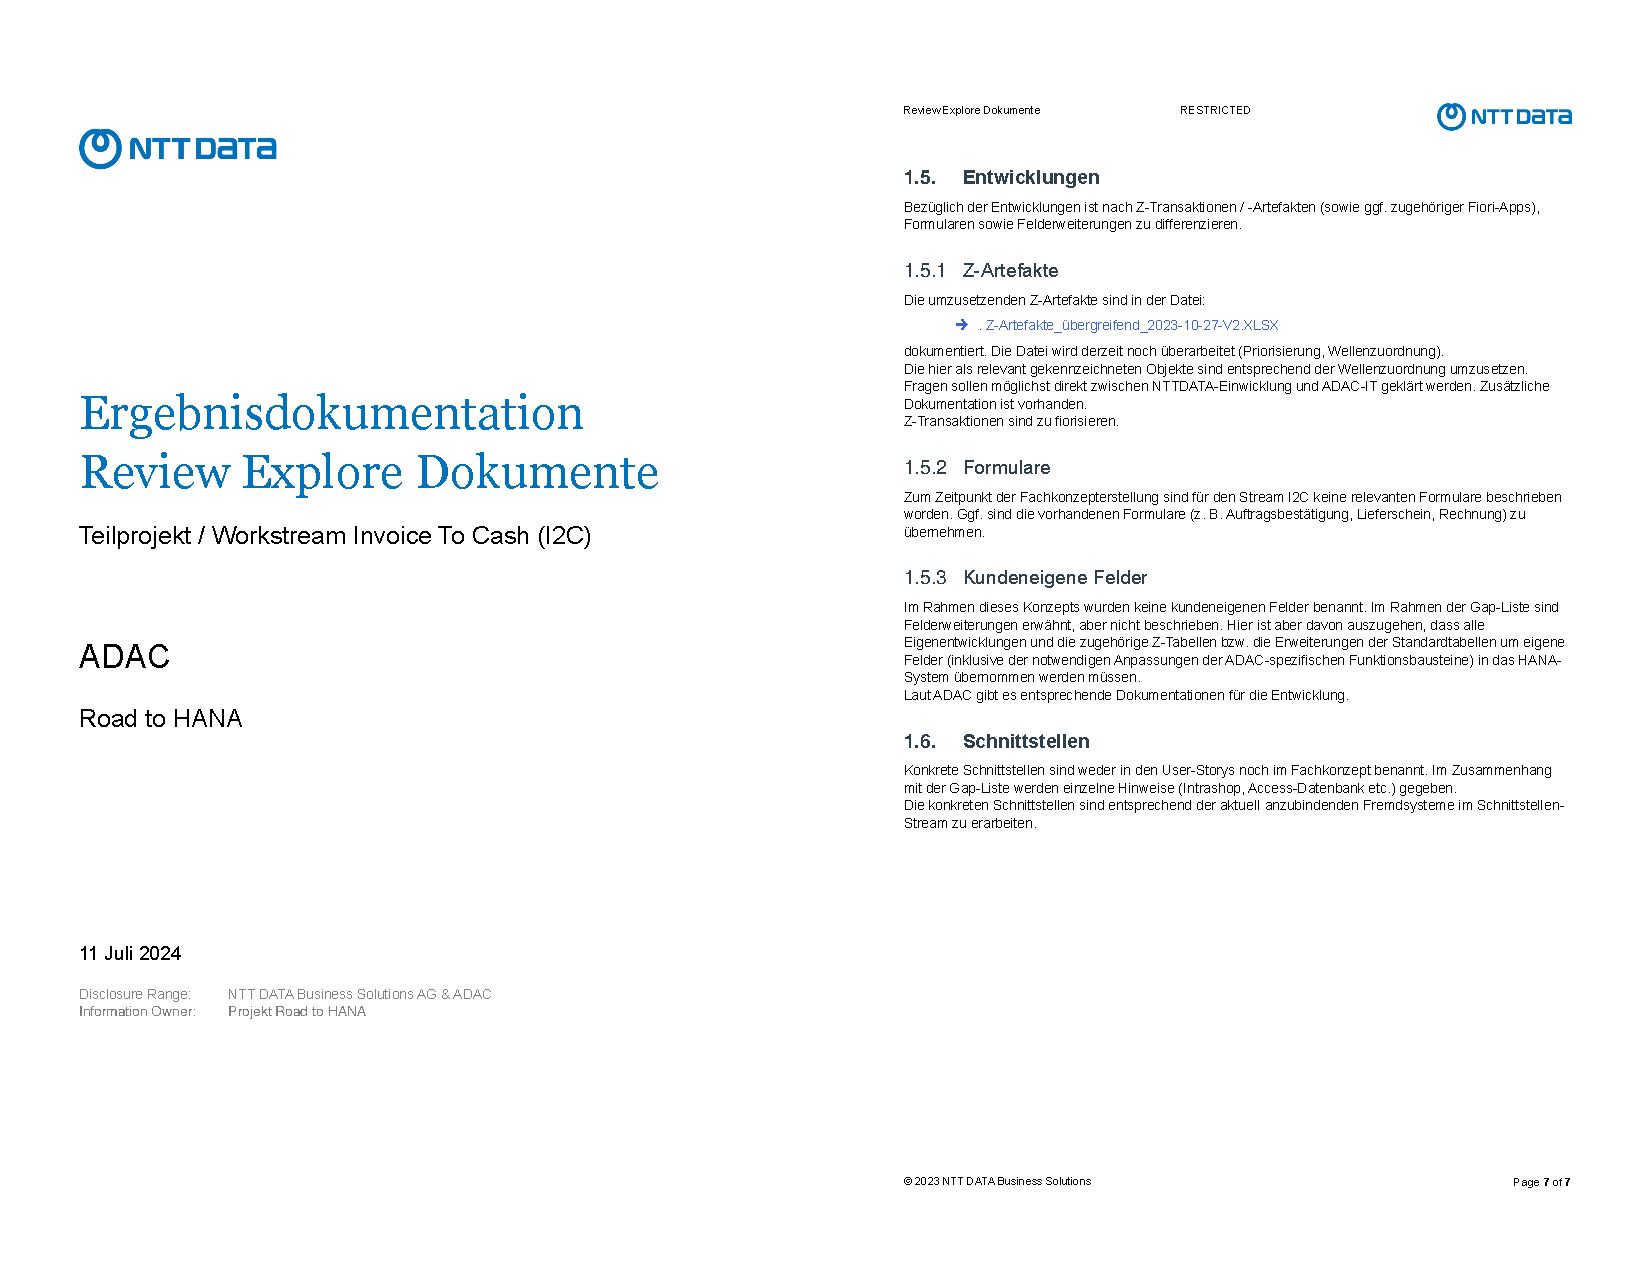
\includegraphics[width=0.99\textwidth]{98_Pictures/R2H_ErgebnisdokumentationStreamI2C.pdf}
    \caption{\acrshort{gu}-Ramp-Up Dokumentation Stream I2C \acrshort{ricefw}+\acrshort{pb}}
     \label{fig:R2HErgebnisdokumentationStreamI2C}
\end{figure}

\newpage